%!TEX root = ../thesis.tex

\section{従来手法}
本研究のベースとなる岡田らの研究について述べる. 先に述べたように, 本論文では岡田らの手法を「従来手法」と呼ぶ. 従来手法は, 地図を用いたルールベース制御器による走行を模倣学習し, 似た行動を画像を用いて行う手法である.\par
\figref{Fig:imitation_sys}に, 経路追従行動を視覚に基づいてオンラインで模倣するシステムを示す. 手法は模倣学習により, 学習器の訓練をする学習フェーズと訓練した結果を検証するテストフェーズにわかれる. なお, 両フェーズで用いる並進速度は一定の値を用いる.

\vspace{3cm}

\begin{figure}[hbtp]
  \centering
 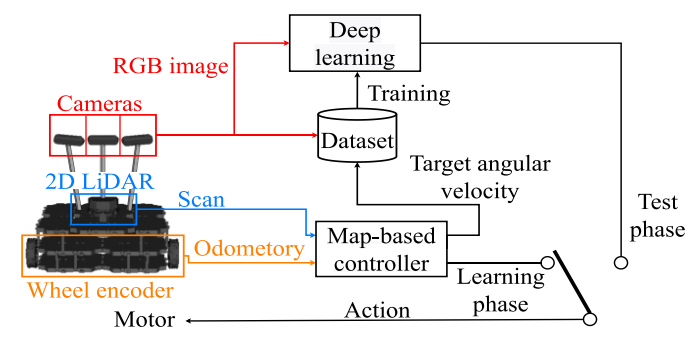
\includegraphics[keepaspectratio, scale=0.5]
      {images/imitation_sys.png}
 \caption{Learning phase of conventional method}
 \label{Fig:imitation_sys}
\end{figure}

\newpage

\subsection{学習フェーズ}
学習フェーズは, 模倣学習によって学習器の訓練を行うフェーズである. 地図を用いたルールベース制御器に, 測域センサとオドメトリのセンサ入力で自律移動する. 具体的には, ROS navigation\_stackパッケージを利用して, ロボットに自律移動させる. 学習フェーズでは, ロボットの中央, 左, 右に傾けて取り付けた3つのカメラを用いて画像を取得する. 一方で, テストフェーズでは, ロボットの中央に取り付けたカメラのみを用いて画像を取得する. 
\par
自律移動させる際に, 取得するデータ量を増加させること及び, 過学習の抑制を目的として, \tabref{table:angular}に示すような処理を行う. また, 地図を用いたルールベース制御器による走行をそのまま模倣学習するのではなく, 少し蛇行するように自律移動させることで, 経路に戻るような挙動も学習できるようになっている. \figref{Fig:dakou}に示すように, 実際にロボットを制御する行動と経路に従う行動を別に扱うことで, 常に経路に従う行動をデータセットに加えることを可能にしている. 
% ロボットに搭載したカメラ画像と地図を用いたルールベース制御器が出力するロボットのヨー方向の角速度の値をデータセットに加える. 
% このデータセットを用いて, リアルタイムに模倣学習を行う. 
\par
岡田らの手法では, データセットの収集方法に種類がある. 
% 本論文では前報\cite{okada2}において最も経路追従の成功率が高い手法を用いて, ロボットに模倣学習をさせる.
本論文では, その中で最も経路追従の成功率が高い手法を用いて, ロボットに模倣学習をさせる.

\begin{table}[hbtp]
  \caption{Angular velocity offset}
  \label{table:angular}
  \centering
  \begin{tabular}{|c|c|}
    \hline
    Left camera  & Angular velocity of a rule-based controller using a map + 0.2 rad/s\\
    \hline
    Center camera  & Angular velocity of a rule-based controller using a map  \\
    \hline
    Right camera  & Angular velocity of a rule-based controller using a map - 0.2 rad/s   \\
    \hline
  \end{tabular}
\end{table}

\begin{figure}[hbtp]
  \centering
 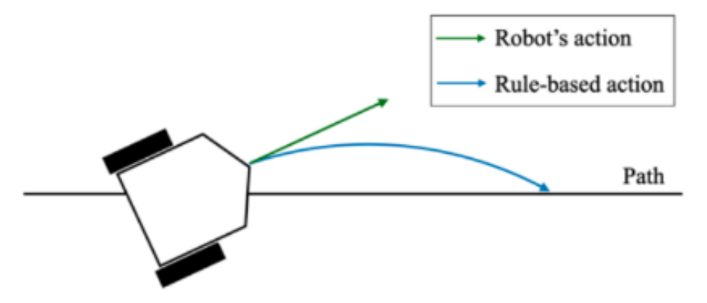
\includegraphics[keepaspectratio, scale=0.38]
      {images/dakou.png}
 \caption{Output of rule-based controller using a map and actual robot behavior from \cite{okada1}}
 \label{Fig:dakou}
\end{figure}

\subsection{テストフェーズ}
学習器の訓練後, \figref{Fig:test_phase}で示すテストフェーズへ移行する. このフェーズでは, 学習器にカメラ画像を入力し, 出力されるヨー方向の角速度を用いて自律移動することで, 訓練後の学習結果を評価する. なお, テストフェーズでは中央のカメラのみを用いる.

\vspace{3cm}


\begin{figure}[hbtp]
  \centering
 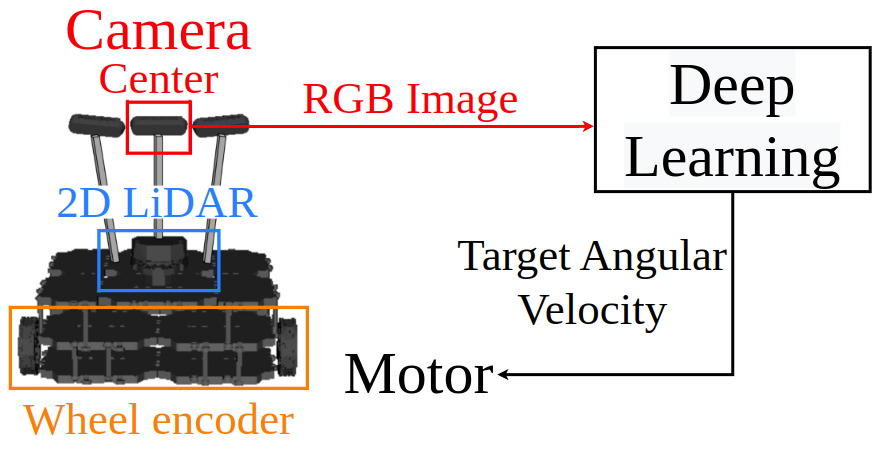
\includegraphics[keepaspectratio, scale=0.4]
      {images/test_phase2.png}
 \caption{Test phase of conventional method}
 \label{Fig:test_phase}
\end{figure}

% \vspace{3cm}

% \subsubsection{etc...}
\newpage